\section{Results}
\label{section:results}

In order to demonstrate the performance of our method, we conducted two sets
of tests.
In the first we simulated observables from a set of stellar parameters for a
few hundred stars using the MIST stellar evolution models and the
gyrochronology model of equation \ref{eqn:gyro}.
The ages predicted with our model were compared to the true parameters used to
generate the data.
In the second we tested our model by measuring the ages of individual stars in
the NGC 6819 open cluster.

\subsection{Test 1: simulated stars}
For the first test we drew masses, ages, bulk metallicities, distances and
extinctions at random for 1000 stars from the following uniform distributions:
\begin{eqnarray}
& \mathrm{EEP} \sim U(198, 480) \\
% & M \sim U(0.5, 1.5)~[M_\odot] \\
& A \sim U(0.5, 14)\mathrm{~[Gyr]} \\
& F \sim U(-0.2, 0.2) \\
& D \sim U(10, 1000)~\mathrm{[pc]} \\
& A_V \sim U(0, 0.1).
\end{eqnarray}
\teff, \logg, \fhat, parallax, and apparent magnitudes $B$, $V$, $J$, $H$, $K$,
\gaia\ $G$, $G_{BP}$ and $G_{RP}$ were generated from these
stellar parameters using the MIST stellar evolution models.
We added a small amount of noise to the `observed' stellar properties in order
to reflect typical observational uncertainties.
We added Gaussian noise with a standard deviation of 25 K to \teff, 0.01 dex
to \feh\ and \logg, and 10 mmags to $B$, $V$, $J$, $H$, and $K$ magnitudes.
The noise added to Gaia $G$-band photometry ranged from
0.3 mmag for stars brighter than 13th magnitude, to 10 mmag for stars
around 20th magnitude \citep{evans2017, brown2018}.
Noise added to \gaia\ $G_{BP}$ and $G_{RP}$ bands ranged from 2 mmag for stars
brighter than 13th magnitude to 200 mmag for stars fainter than 17th.
Unphysical combinations of stellar parameters were discarded, resulting in a
final sample size of 841 simulated stars.
Figure \ref{fig:CMD_age} shows the position of these stars on an HRD
(with \logg\ on the y-axis instead of luminosity to improve the visibility of
the MS), colored by their age.
Rotation periods for FGK and early M dwarfs were generated using the
gyrochronology relation of equation \ref{eqn:gyro}.
Rotation periods for these stars were generated using the gyrochronology
relation described in equation \ref{eqn:gyro}.
We added a conservative value of 10\% Gaussian noise to all stellar
rotation periods.
This is a rather crude approximation for the noise distribution of rotation
periods which can be highly non-Gaussian \citep[\eg][]{aigrain2015,
angus2018}.
\begin{figure}
  \caption{
      The simulated star sample plotted on an HRD, colored by age
    (top panel) and rotation period (bottom panel).
    HRD positions were calculated using MIST isochrones via the {\tt
    isochrones.py} {\it Python} package and rotation periods were generated
    using equation \ref{eqn:gyro}.
    This figure was generated in a Jupyter notebook available at
    \url{https://github.com/RuthAngus/stardate/blob/master/paper/code/Simulate_data.ipynb}
}
  \centering
    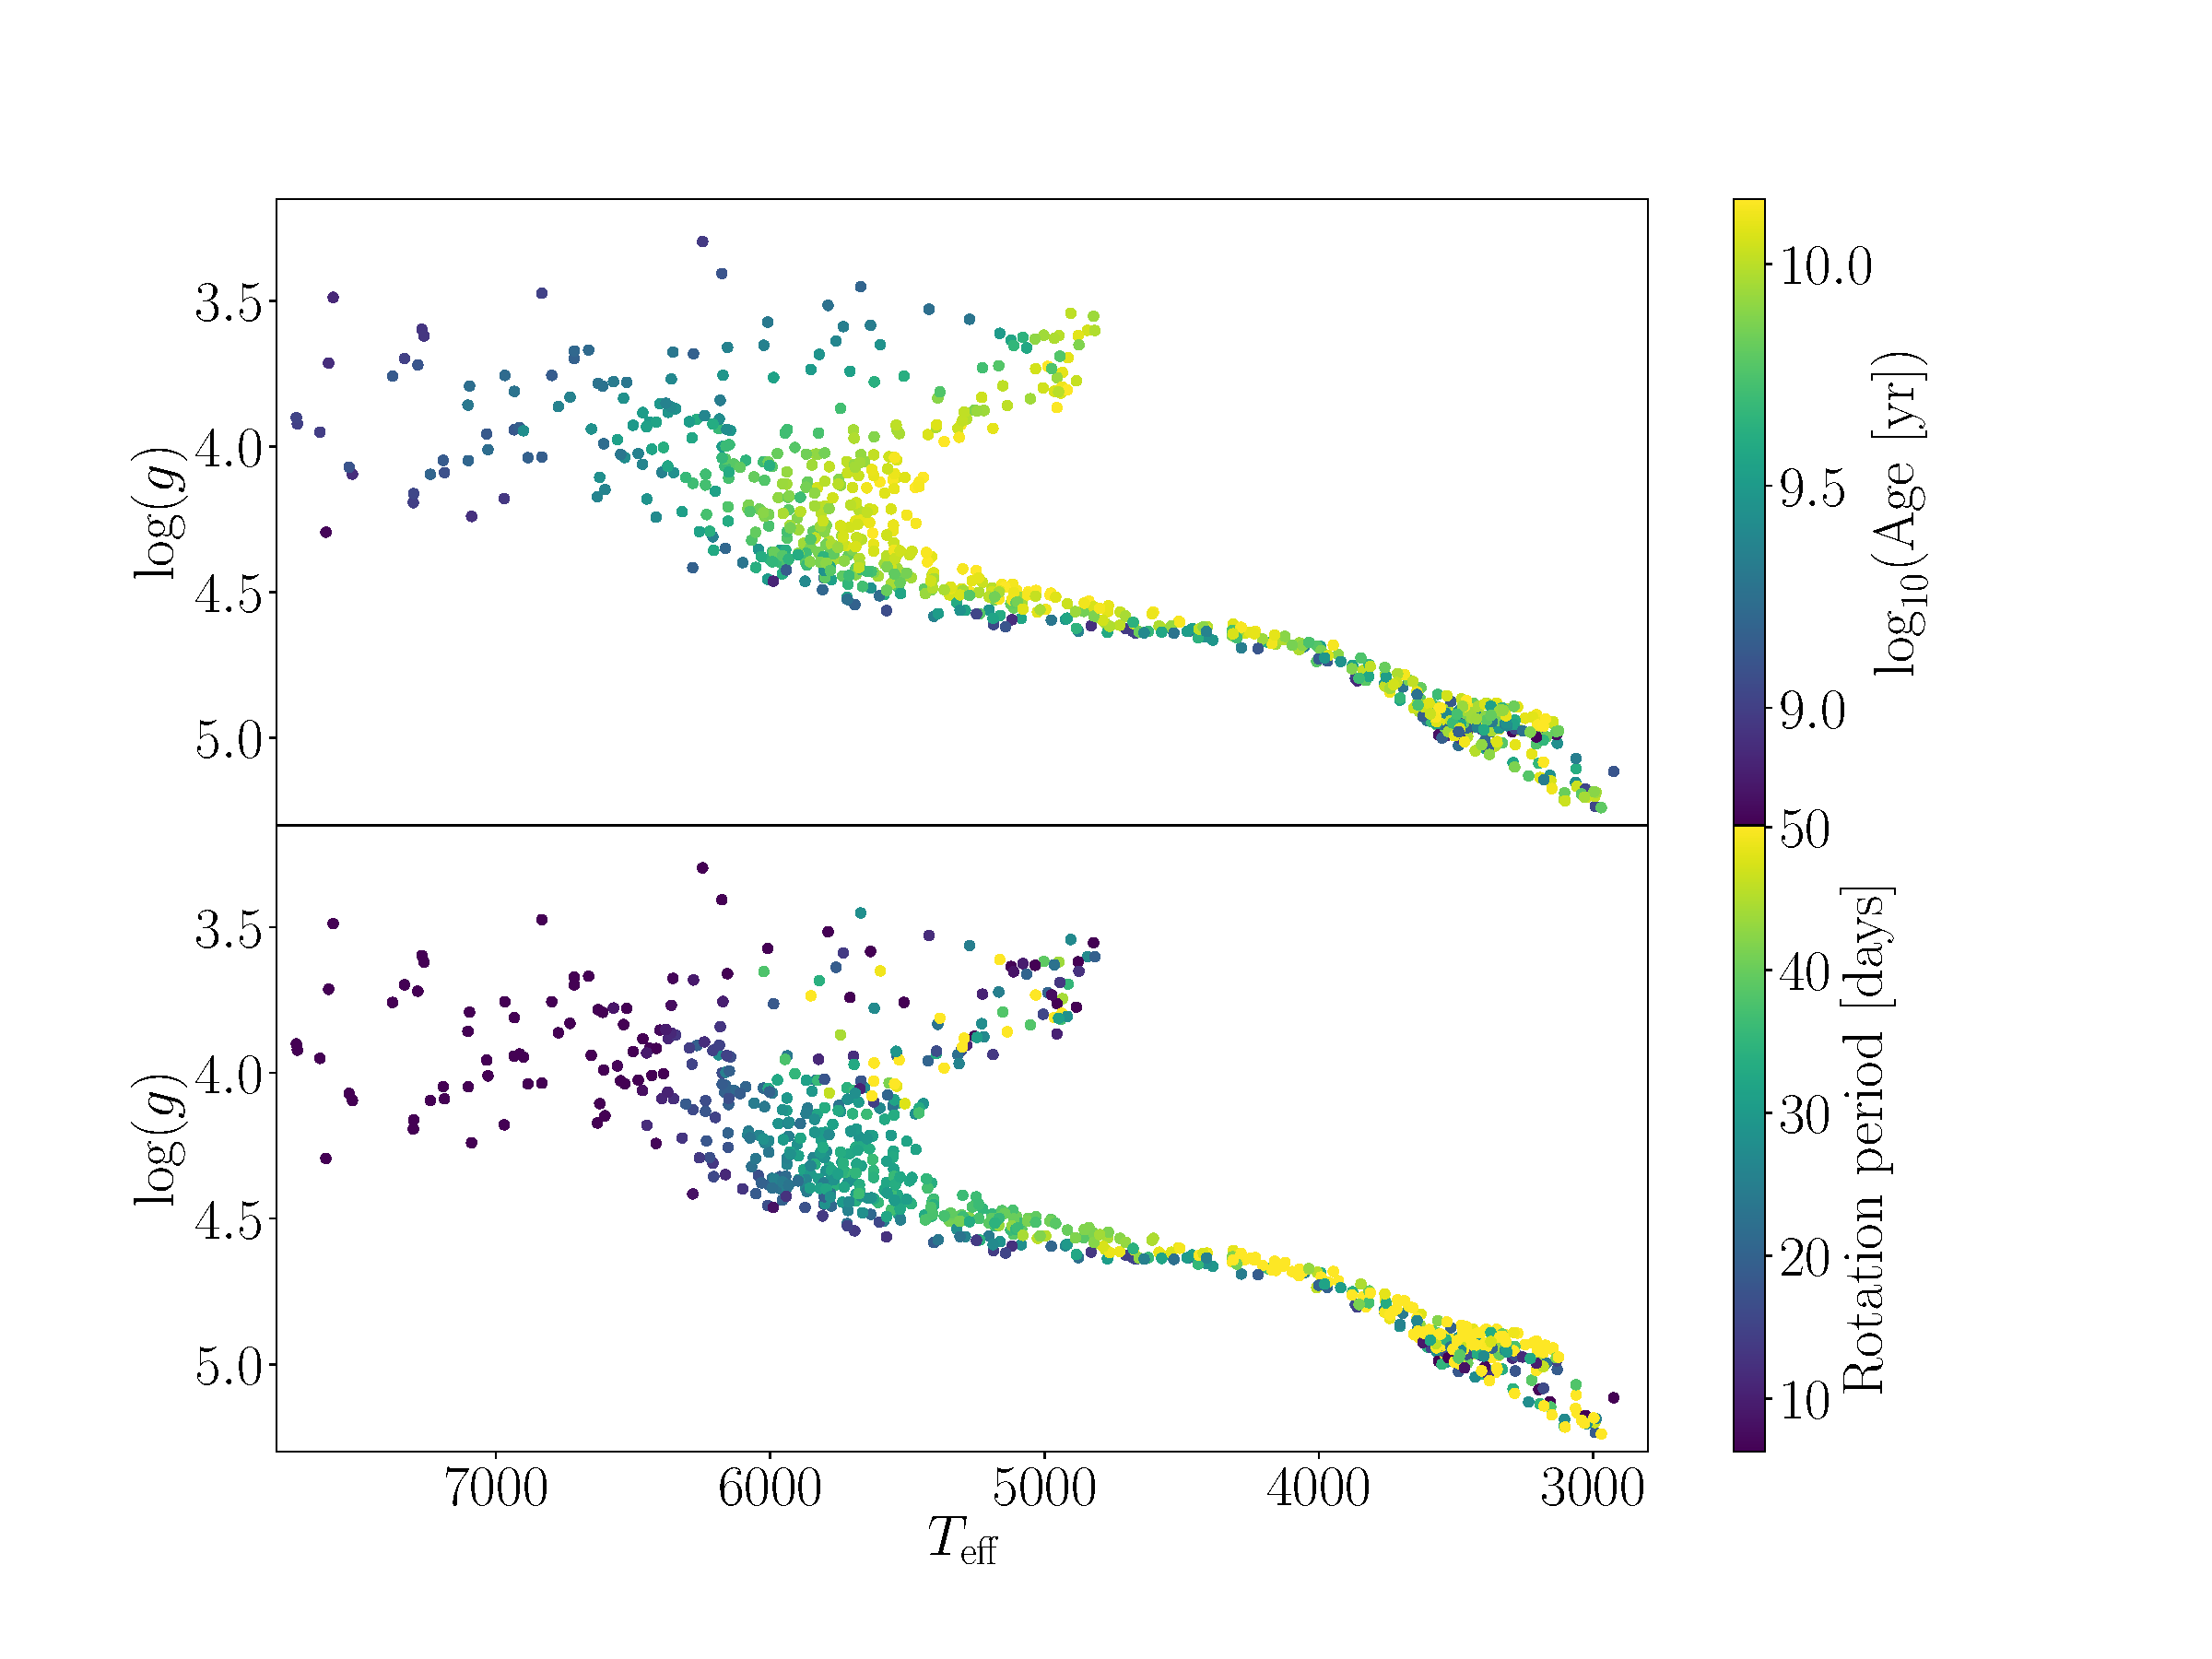
\includegraphics[width=1\textwidth]{simulated_CMD}
\label{fig:CMD_age}
\end{figure}
Figure \ref{fig:rotation_model} shows the rotation periods of 841
stars generated from the gyrochronology model.
\begin{figure}
  \caption{
The rotation period model.
    Late F, GK and early M dwarfs (stars with 0.56 $<$ \gcolor\ $<$ 2.7 follow
    the Praesepe-calibrated gyrochronology relation (dashed gray lines), with
    the exception of old, slowly
    rotating stars with large Rossby numbers whose rotation periods are fixed
    at 2$\times$ their convective overturn time.
    The rotation periods of early F (\gcolor $<$ 0.56), late M dwarfs (\gcolor
    $<$ 2.7) and subgiants (EEP $>$ 454) were generated
    from a log-normal distribution with standard deviation shown in figure
    \ref{fig:variance}.
% The top panel shows the rotation periods vs. B-V colors of simulated stars,
The top panel shows the rotation periods vs. \gcolor\ colors of simulated stars,
    colored by their age and the bottom panel shows the same stars colored
    by their equivalent evolutionary point (EEP).
    % 9, 11, and 13 (rotation periods rise with age).
    The gray lines describe the mean gyrochronology model at ages 1,
    3, 5, 7, 9, 11, and 13 (rotation periods rise with age).
}
  \centering
    \includegraphics[width=1.\textwidth]{rotation_model_praesepe}
\label{fig:rotation_model}
\end{figure}

We took two approaches to inferring the ages of these simulated stars:
firstly using isochrone fitting {\it only}, and secondly using isochrone
fitting {\it combined with} a gyrochronology model (\sd).
Since the posterior PDFs of stars are often not unimodal, we found that the
choice of initial positions of the {\tt emcee} walkers influenced the final
outcome because walkers occasionally got stuck in local minima.
We found that the following set of initial parameters worked well, though not
perfectly, for FGK dwarfs but sacrificed some accuracy in subgiant ages: EEP =
330, $A = 9.56$ Gyr, $F = -0.05$, $D = 269$ pc and $A_V = 0.0$.
Figure \ref{fig:simulation_results} shows the results of combining
gyrochronology with isochrone fitting for the simulated sample.
The stars' true ages are plotted against their predicted ages, with \sd\ ages
in color, and ages predicted using isochrone fitting only plotted in light
grey.
The five panels show the results for five different types of stars: late F, GK
and early M dwarfs which are still undergoing magnetic braking (Ro $<$ 2),
late F, GK and early M dwarfs that have ceased magnetic braking (Ro $>$ 2),
% hot stars ($B-V < 0.45$), cool stars ($B-V > 1.4$) and evolved stars (EEP $>$
hot stars (\gcolor\ $<$ 0.56), cool stars (\gcolor\ $>$ 2.7) and evolved stars
(EEP $>$ 454).
As expected, the low $Ro$, FGK stars show the most dramatic improvement in age
precision.
\racomment{Summary statistics rewrite in progress...}
\begin{figure}
  \caption{
The true vs. predicted ages of simulated stars.
    Ages calculated by combining gyrochronology
    and isochrone fitting with \sd are shown in color and ages calculated with
    isochrone fitting only are shown in gray.
The five panels show the results for five different groups of stars: low $Ro$
late F, GK and early M dwarfs, high $Ro$ late F, GK and early M dwarfs, early
    F stars (\gcolor\ $<$ 0.56), late M dwarfs (\gcolor\ $>$ 2) and subgiants
    (EEP $>$ 454).
Gyrochronology is highly effective for low $Ro$ late F, GK and early M dwarfs
and somewhat effective for high $Ro$ late F, GK and early M dwarfs.
Ages for other groups were improved slightly but not substantially.
% Outliers are caused by multimodal posterior PDFs and imperfect MCMC sampling.
}
  \centering
    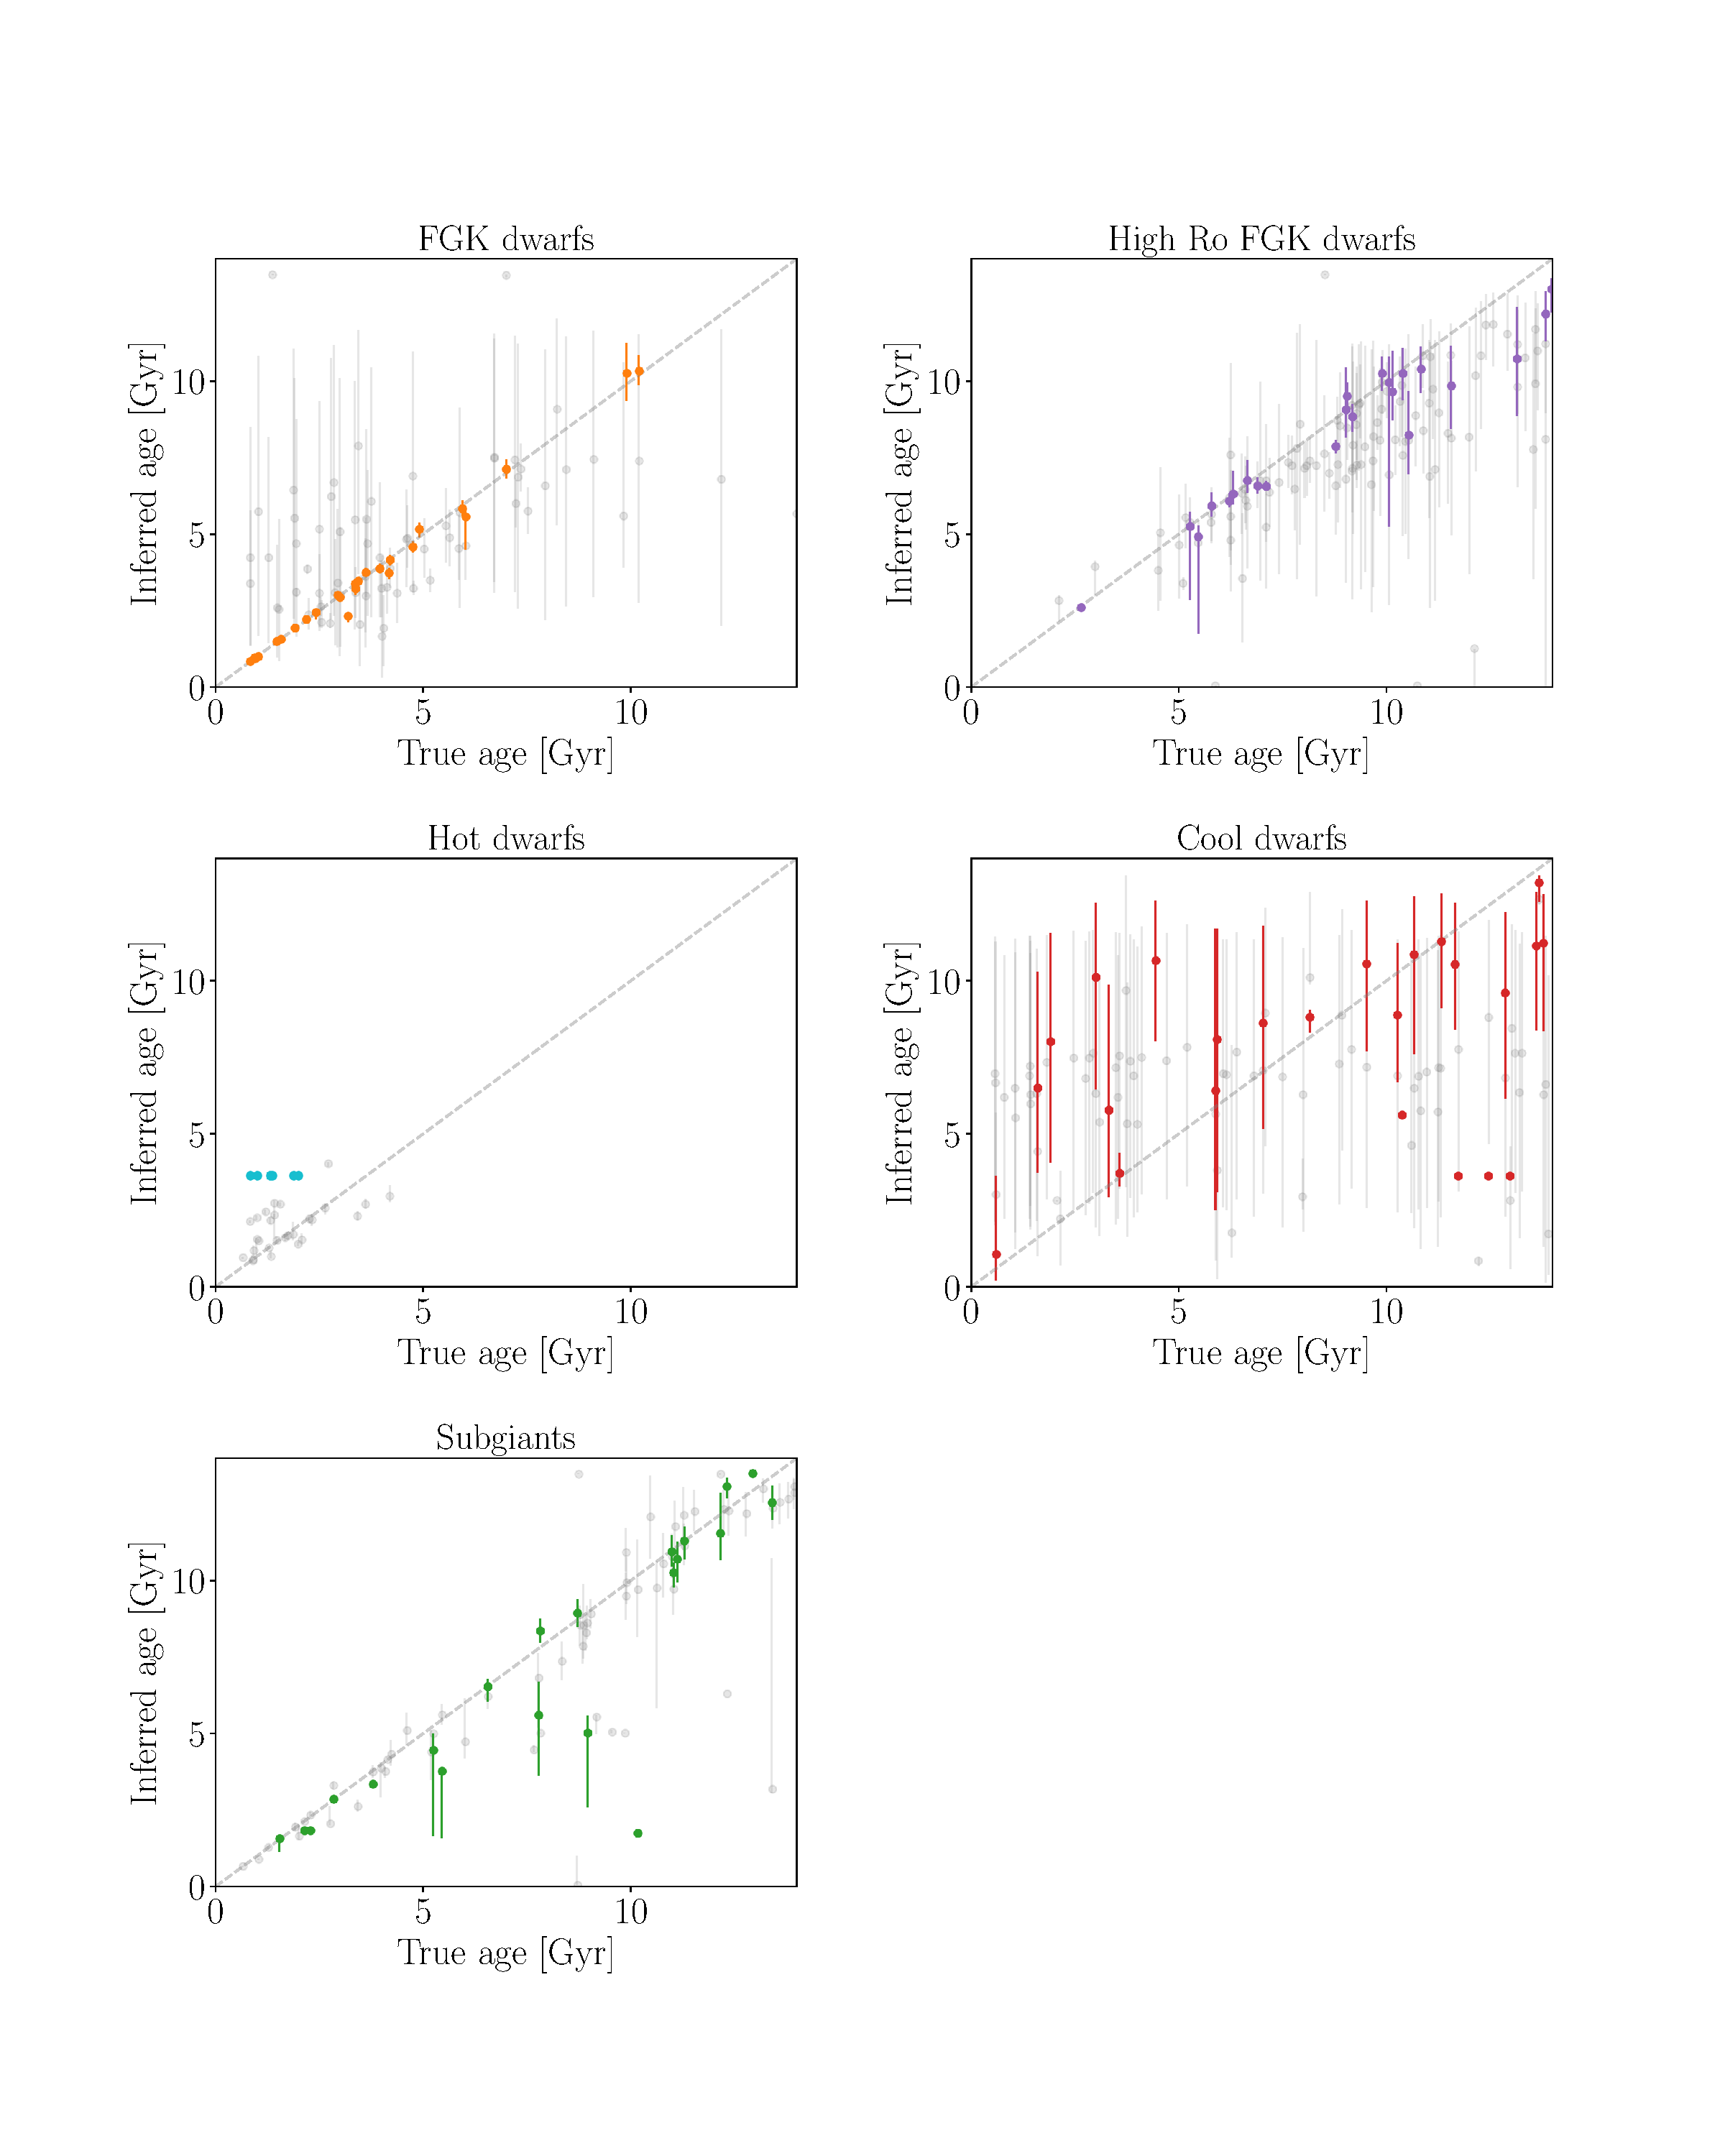
\includegraphics[width=1\textwidth]{simulation_results}
\label{fig:simulation_results}
\end{figure}

Figure \ref{fig:precision} shows the simulated stars on an HRD, with
points colored by the relative precision of their predicted ages.
The top panel shows the precision of ages calculated using both gyrochronology
and isochrone fitting with \sd\ and the bottom panel shows the precision of
ages calculated with isochrone fitting only.
Although these uncertainties are noisy (they are computed from the standard
deviation of the age posteriors) they show that combining gyrochronology and
isochrone fitting improves age precision on the MS
This simulation experiment is optimistic because data were simulated from the
same gyrochronology model used to infer ages, so the results for FGK dwarfs
are extremely accurate by design.
\sd\ can provide precise ages with the caveat that the currently implemented
gyrochronology model is not perfectly calibrated and ages will only be as
accurate as the model.
\begin{figure}
  \caption{
Simulated stars on an HRD, colored by their relative age precision
    using gyrochronology and isochrone fitting via \sd\ (top panel) and
    isochrone fitting only (bottom panel).
Combining gyrochronology with isochrone fitting significantly improves stellar
    age precision on the MS.
Isochrone fitting provides precise ages for hot stars and subgiants and the
    rotation periods of these stars are relatively uninformative, so
    gyrochronology does not significantly improve their age precision.
The ages of late M dwarfs are highly imprecise because their ages are not well
    determined by either their rotation periods or their position on the HRD
    or CMD.
}
  \centering
    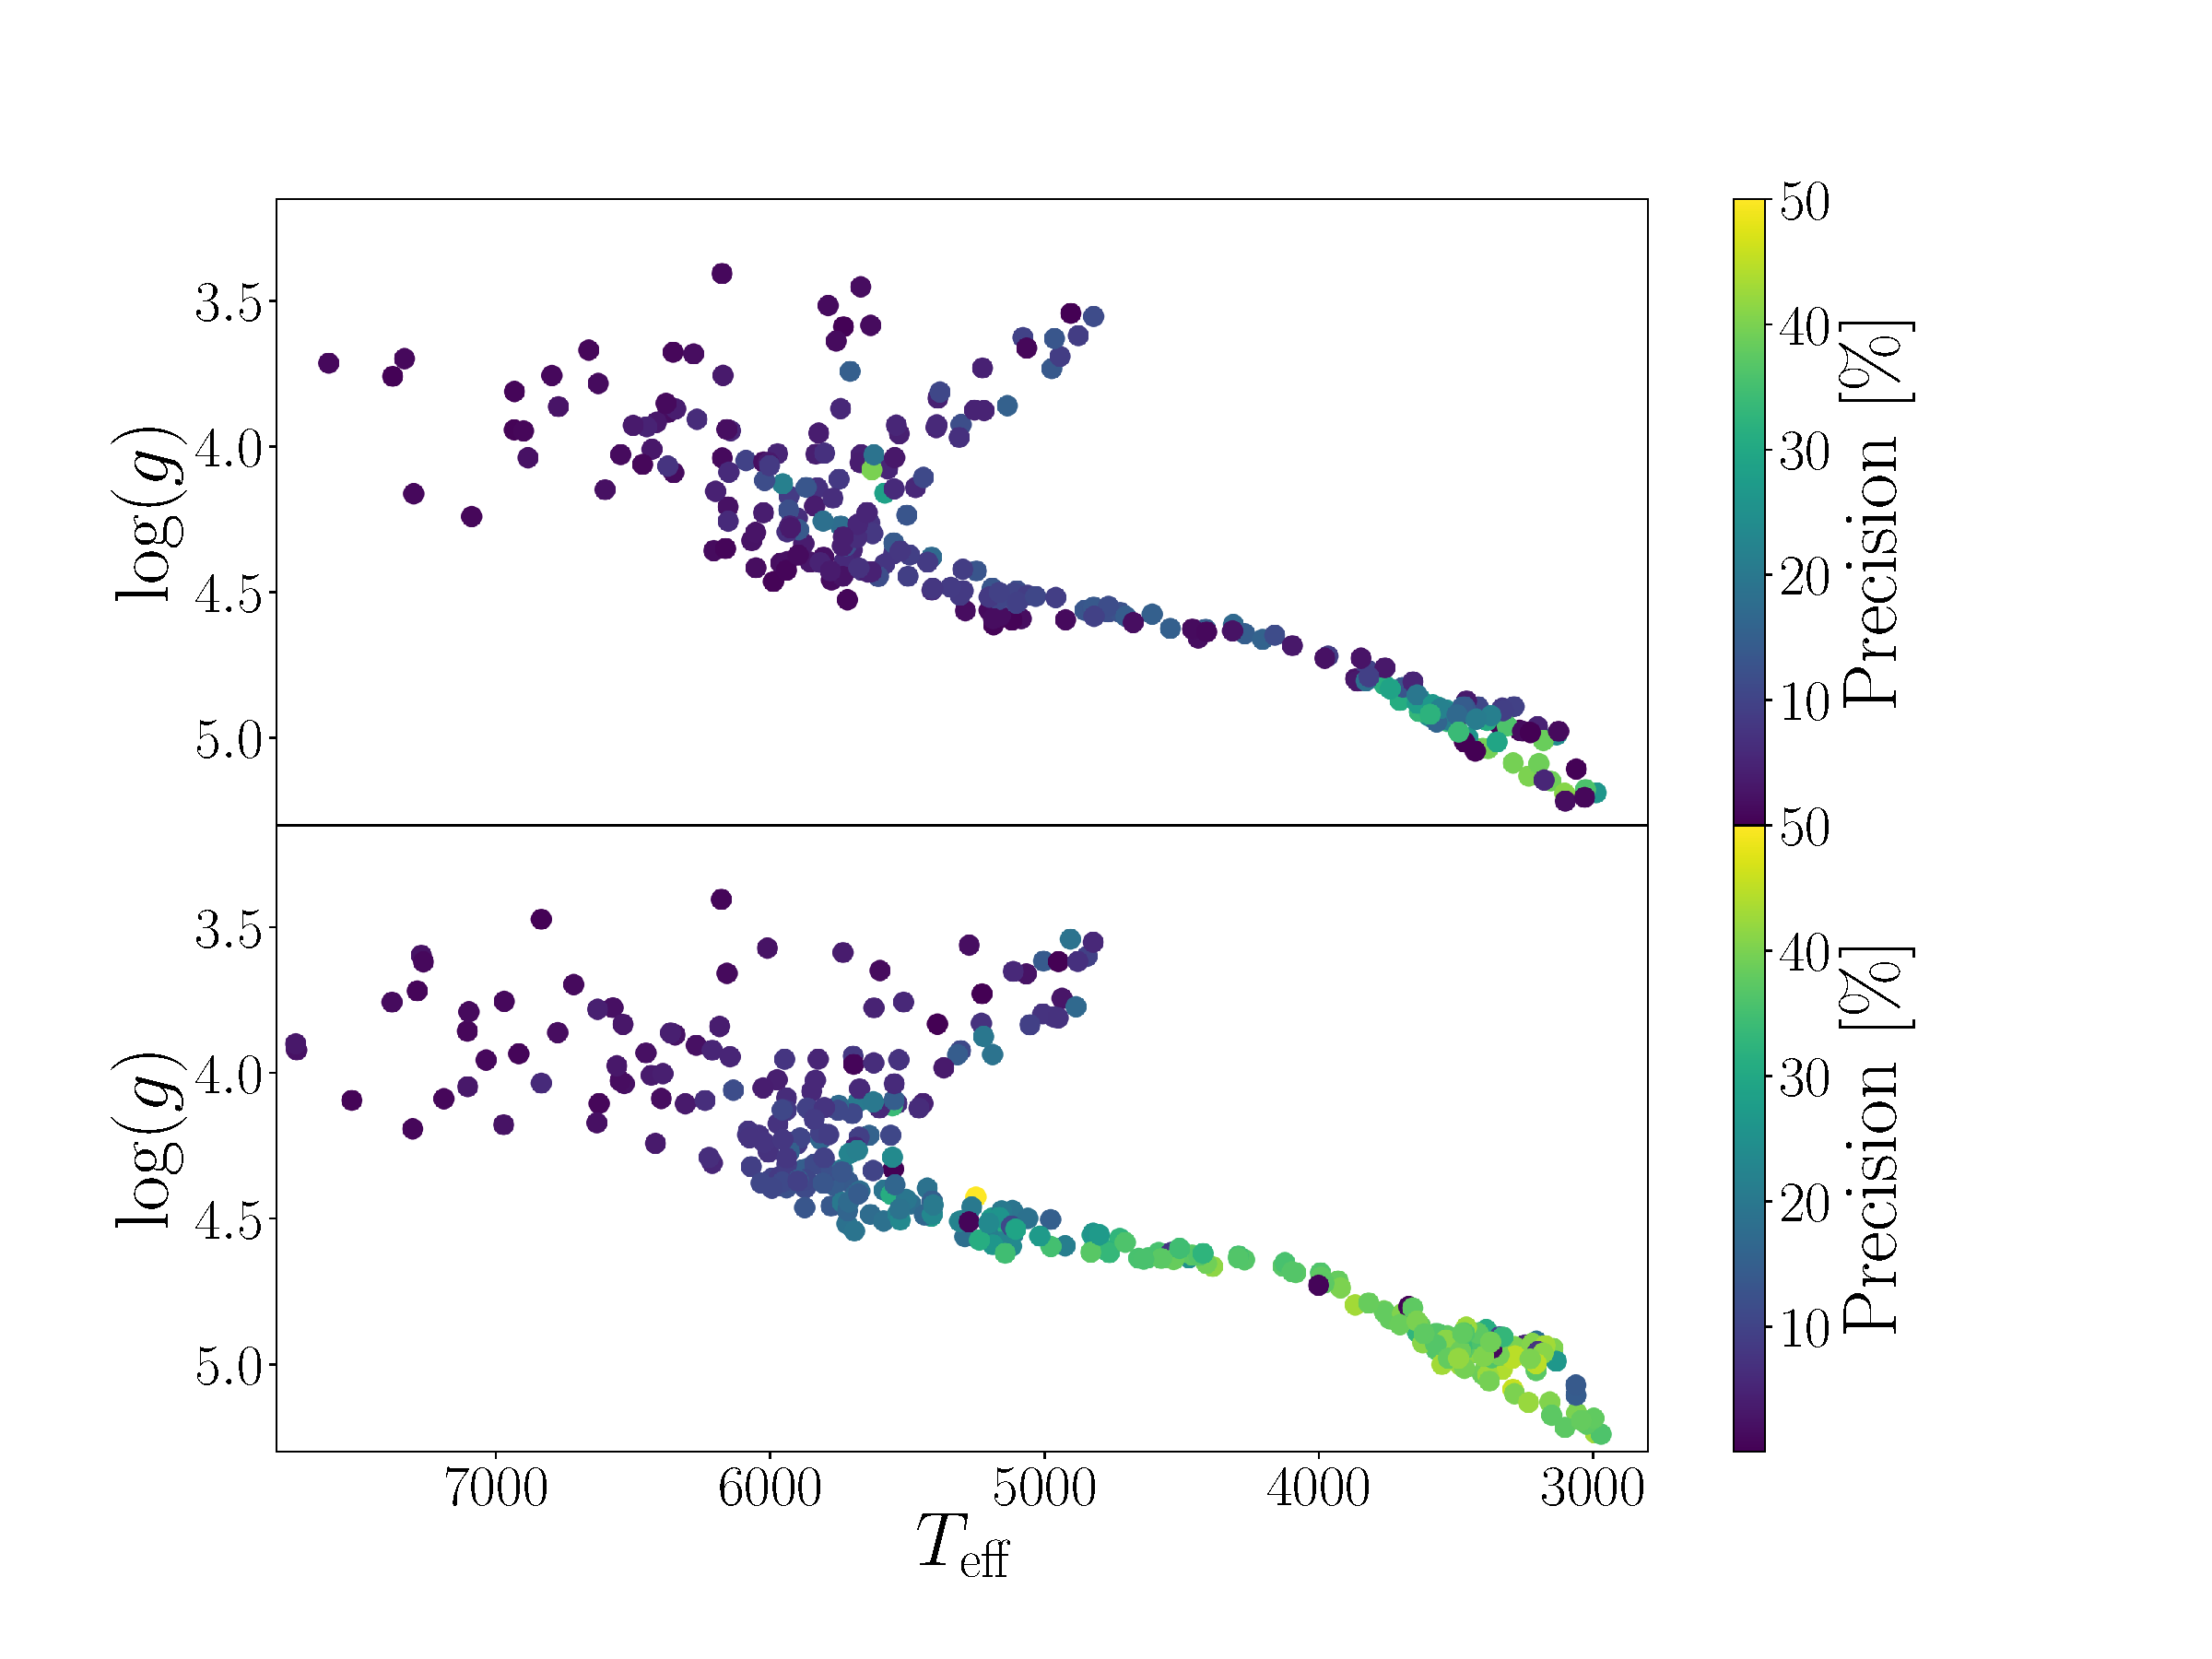
\includegraphics[width=1\textwidth]{precision_plot}
\label{fig:precision}
\end{figure}

\subsection{Test 2: Open clusters}
\racomment{
In order to test our model on real stars with known ages, we selected a sample
of stars in the 2.5 Gyr NGC 6819 cluster.
We compiled \kepler-based rotation periods \citep{meibom2015}, \Gaia\
photometry and \gaia\ parallaxes for members of the NGC 6819 cluster.
Figure \ref{fig:NGC6819} shows the rotation period-color relation of this
cluster and figure \ref{fig:NGC6819_results} shows the results of inferring
the ages of individual cluster members using \sd\ and isochrone fitting.
The ages of F stars in this cluster (\gcolor\ $\sim$ 5.5-6.5) are relatively
precisely constrained by isochrone fitting alone because, at 2.5 Gyr, they are
approaching MS turn-off.
The \sd\ and isochrone-only ages are consistent for this group of stars and
similarly precise, showing that isochrones provide a lot of age information
for these stars and rotation periods do not add significantly more
information.
The G and early K stars in this cluster (\gcolor\ $\lesssim$ 6.5) are not
precisely recovered from isochrone fitting alone -- the isochrone-only age
posteriors tend towards the prior which is a uniform distribution between 0
and 13.8 Gyrs.
In contrast, the rotation periods of G and K stars in this cluster
significantly improve the accuracy of age measurements.
The median age of stars in this cluster was 2.63 $\pm$ 0.16 Gyr when ages were
inferred with a combination of isochrone fitting and gyrochronology, with a
Praesepe-calibrated gyrochronology model.
The previously-calibrated \citet{angus2015} model resulted in a median age of
2.66 $\pm$ 0.21 Gyr.
The median age of the cluster, calculated with isochrone fitting and a
Praesepe-calibrated gyrochronology model, without correcting the photometry
for redenning, was slightly under-estimated at 1.86 $\pm$ 0.22 Gyr.
This suggests that, despite the fact that V-band extinction is a parameter
that gets marginalized over during the inference process, correcting for
extinction {\it before} ages are estimated will reduce bias introduced by
dust.
Finally, the median age of stars in the cluster was 4.27 $\pm$ 0.48 Gyr when
only isochrone fitting was used.
Isochrone-only ages were over-estimated because they were prior dominated, and
the prior was a uniform distribution between 0 and 13.8 Gyr.
\begin{figure}
  \caption{
    The \kepler-based rotation periods of members of the 2.5 Gyr NGC 6819 open
    cluster.
    The raw \gcolor\ colors are shown in red and the dust-corrected colors are
    shown in black.
    The dashed line shows a gyrochronology model that was fit to the Praesepe
    cluster and the Sun in this work, interpolated to 2.5 Gyrs.
    This model was used to infer the ages of these stars.
    For comparison, the solid blue line shows a previously calibrated
    gyrochronology model \citep{angus2015}.
}
  \centering
    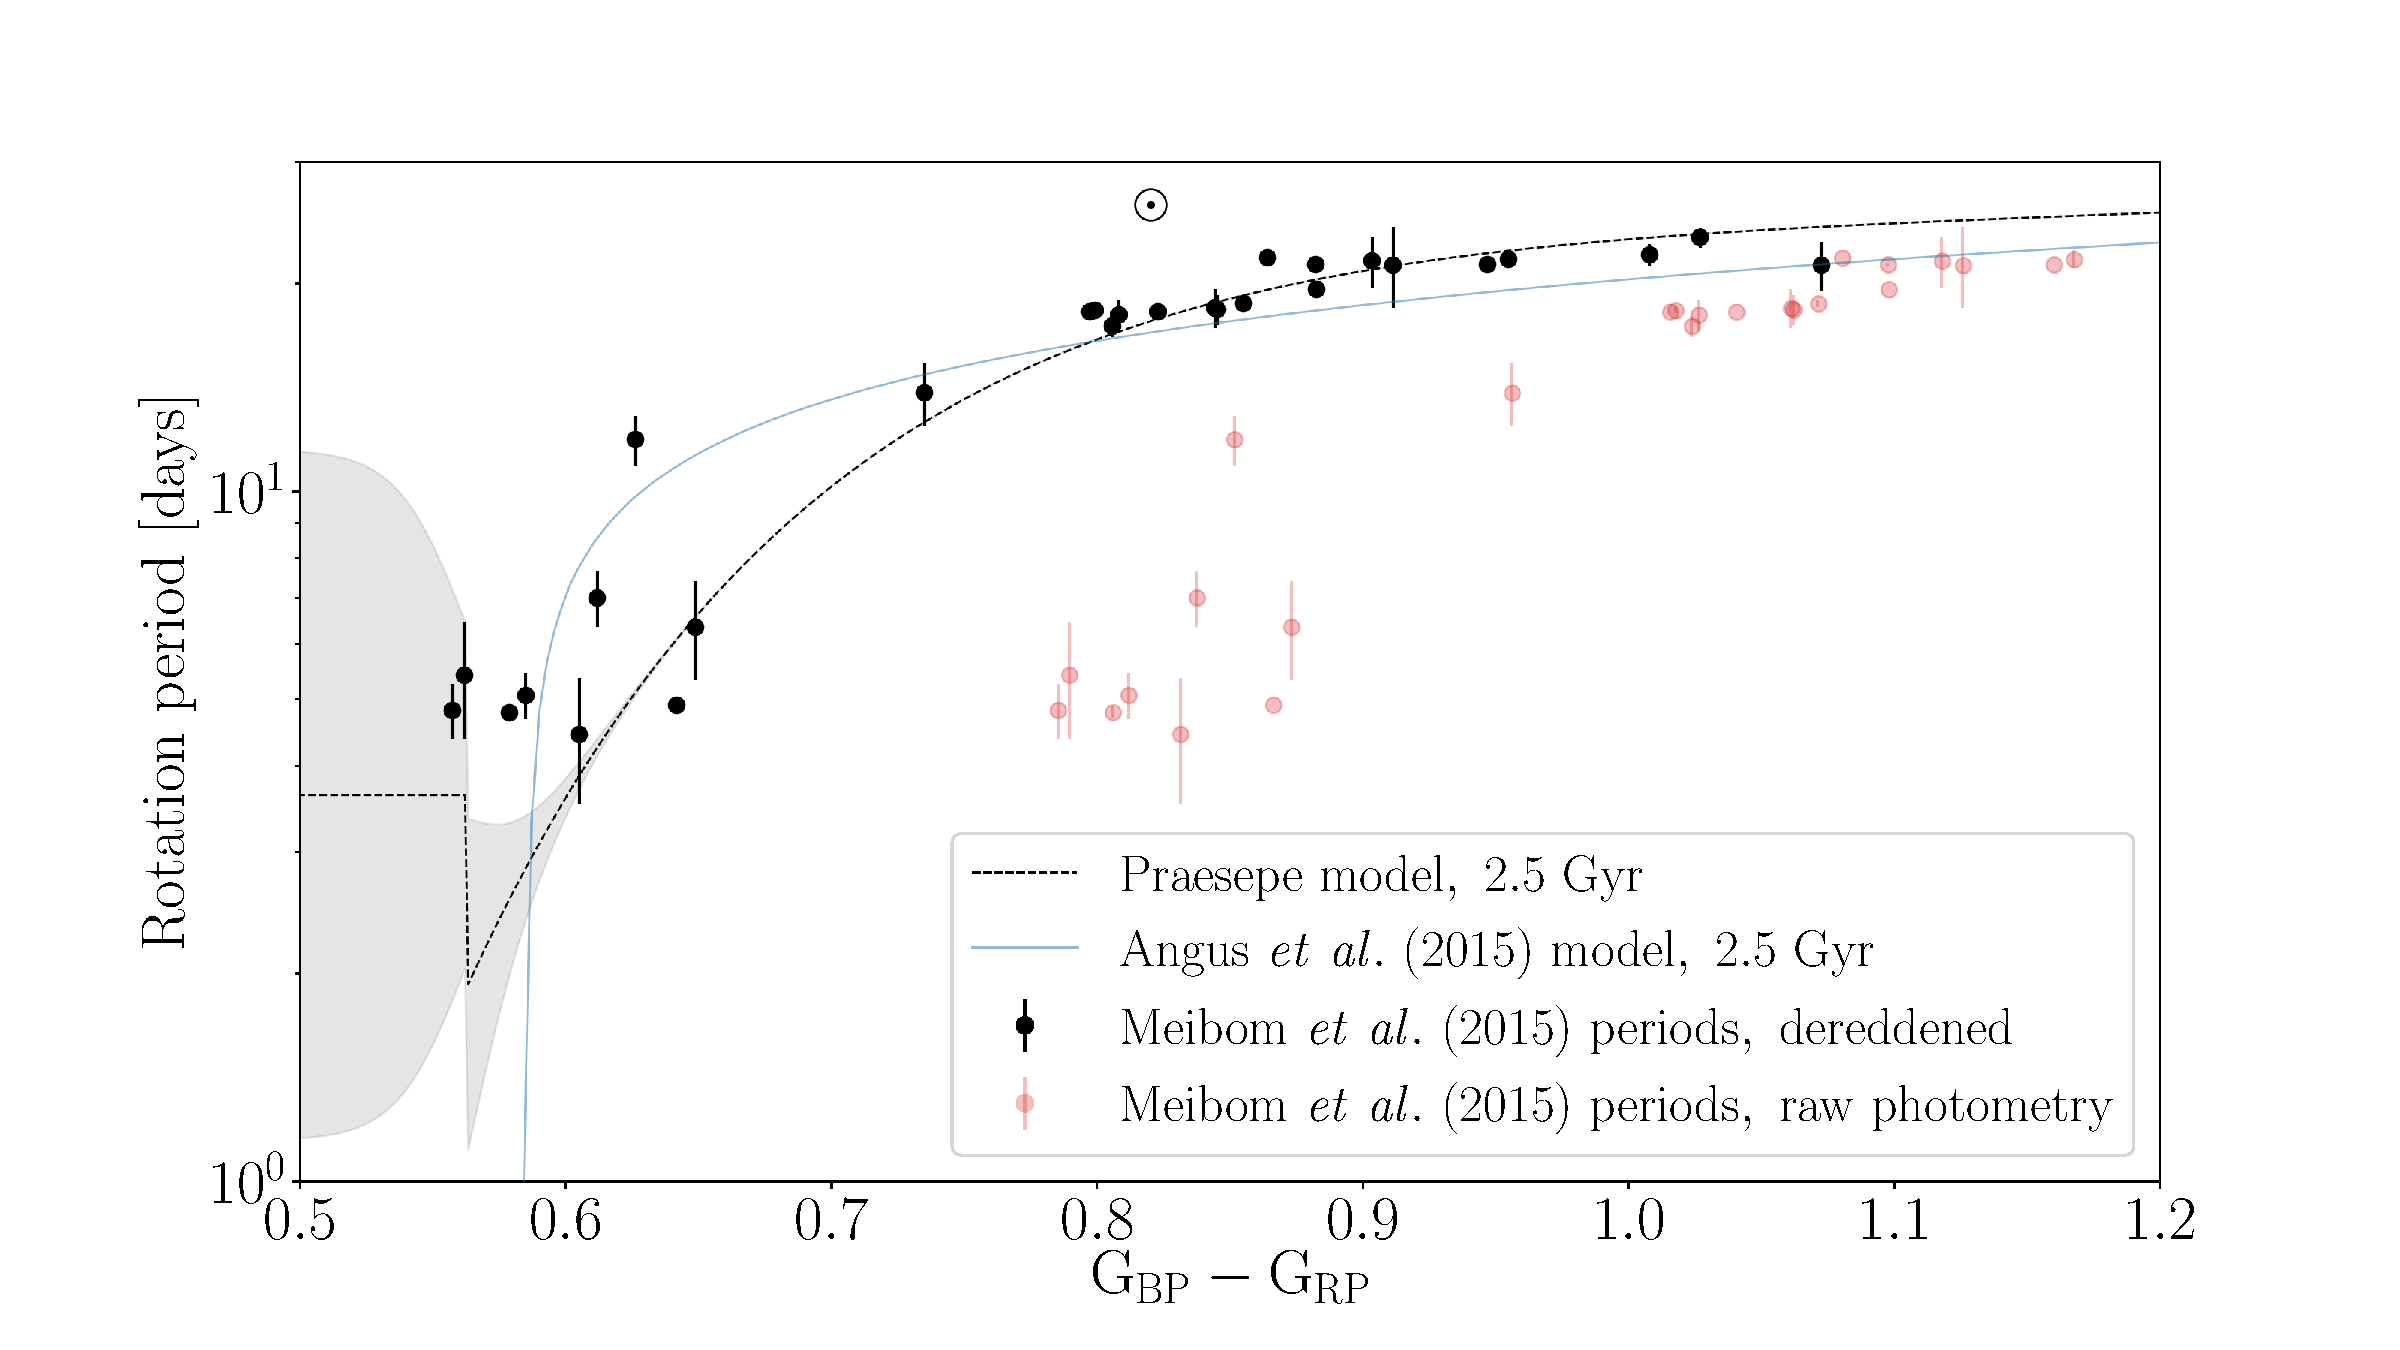
\includegraphics[width=1\textwidth]{NGC6819}
\label{fig:NGC6819}
\end{figure}
\begin{figure}
  \caption{
    The inferred ages of members of the NGC 6819 open cluster as a function of
    their \gcolor\ color.
    Black circles and red squares show the ages of stars inferred using a
    combination of isochrone fitting and gyrochronology, with a gyrochronology
    relation that was calibrated to Praesepe and the Sun.
    Black circles show ages inferred with dereddened \gaia\ $G$, $G_{BP}$ and
    $G_{RP}$ photometry and red squares show ages inferred with uncorrected,
    raw, photometry.
    Even though V-band extinction is marginalized over in the inference
    process, reddening can still bias ages.
    Blue triangles, pointing down show ages inferred using isochrone fitting
    and gyrochronology, with the \citet{angus2015} gyrochronology model.
    Orange triangles show ages inferred using isochrone fitting only.
    The ages of F stars (stars bluer than 0.7) were precisely constrained by
    isochrones and including gyrochronology makes little difference to their
    inferred ages.
    The ages of G and K dwarfs (stars redder than 0.7) were improved in both
    precision and accuracy by including gyrochronology.
    The average age of stars, inferred using the gyrochronology model
    calibrated to Praesepe and the Sun (black circles) was 2.65 $\pm$ 0.13
    which is consistent with the established cluster age.
}
  \centering
    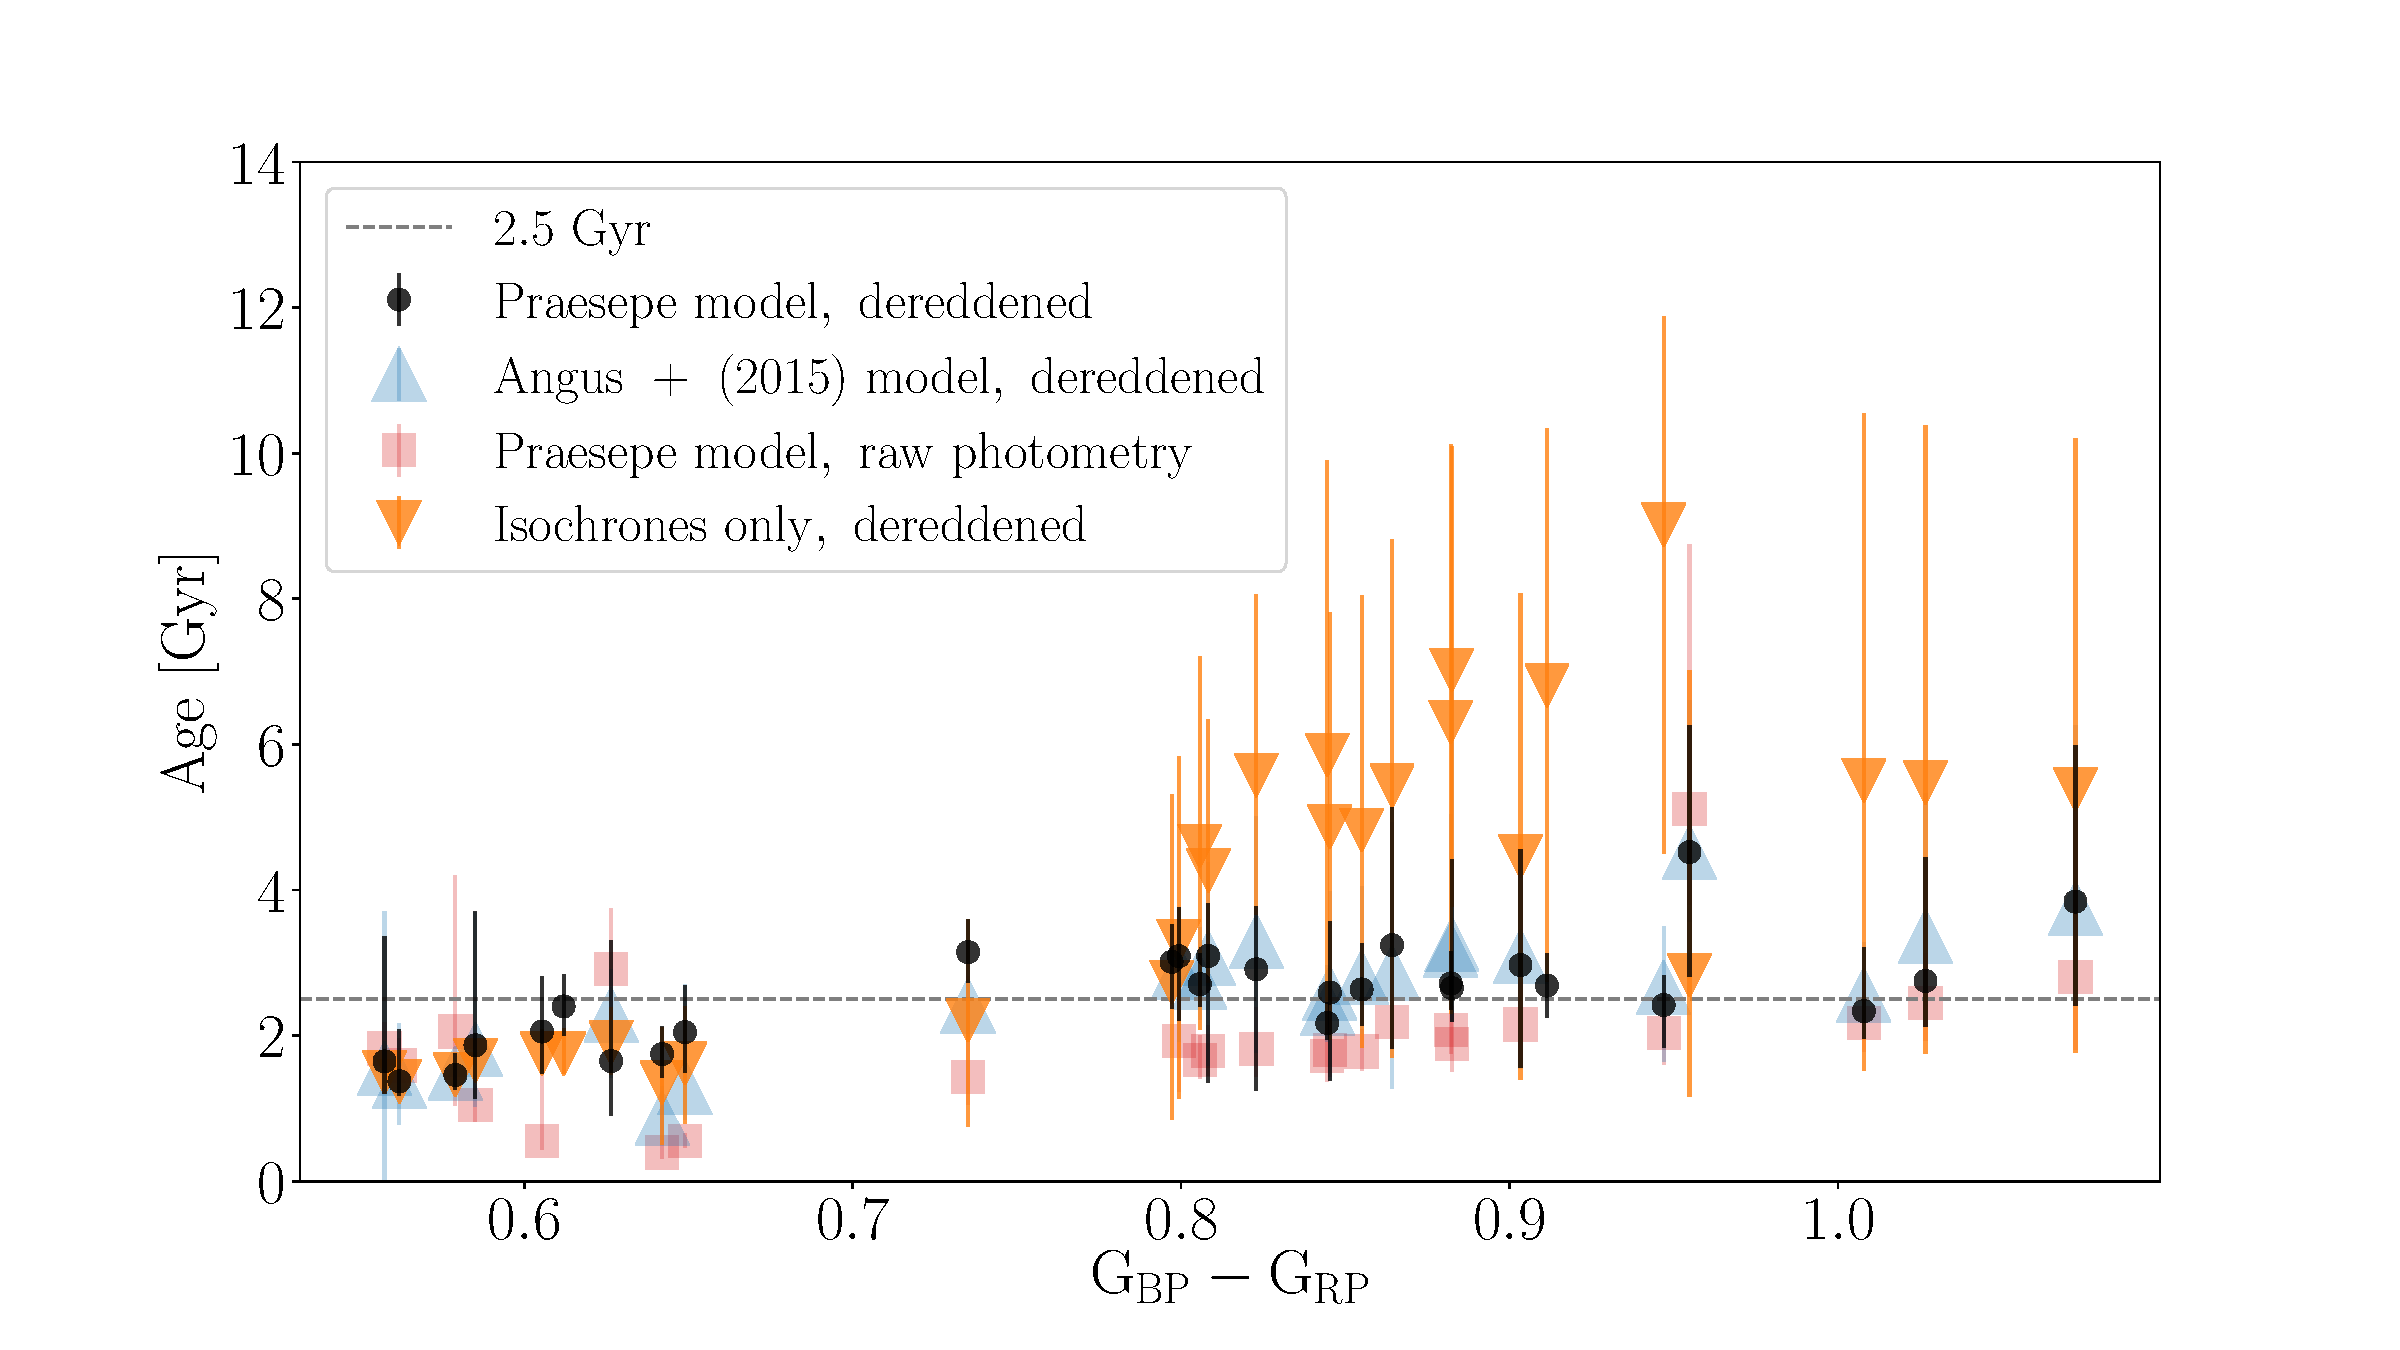
\includegraphics[width=1\textwidth]{NGC6819_results}
\label{fig:NGC6819_results}
\end{figure}

We found that 5\% rotation period uncertainties resulted in the most accurate
ages for NGC 6819.
The uncertainties on the measured rotation periods, provided in
\citet{meibom2015} and shown in figure \ref{fig:NGC6819}, were underestimated
for some stars.
Underestimating the rotation period uncertainty can result in an inaccurate
age estimate.
This raises the question: how should uncertainties on rotation periods be
estimated?
The likelihood is weighted by the inverse variance, so uncertainties on the
rotation period control the relative information provided by gyrochronology,
isochrones, and the prior.
If rotation period uncertainties are either too large or too small, the
resulting age estimate will be imprecise and/or inaccurate.
It is difficult to measure uncertainties on rotation periods directly because
standard techniques such as Lomb-Scargle periodograms and autocorrelation
functions do not have a reliable way to calculate realistic uncertainties.
In general, rotation period uncertainties should probably be calculated
empirically via simulations as in the \citet{aigrain2015} study.
A thorough exploration of how rotation period uncertainties affect stellar
ages via gyrochronology would be useful in future.}
